\documentclass[12pt]{article}
\usepackage{amssymb,mathtools}
\usepackage[margin=1in]{geometry}
\usepackage{fancyhdr}
\usepackage{circuitikz}
\usepackage{graphicx}
\graphicspath{ {./Figures/} }
\usepackage{amsmath}
\usepackage{ragged2e}
\usepackage{subcaption} 
\usepackage{float}
\usepackage{cancel}
\usepackage{siunitx}
\pagestyle{fancy}
\usepackage[shortlabels]{enumitem}
\usepackage{mathtools}
\newcommand*{\permcomb}[4][0mu]{{{}^{#3}\mkern#1#2_{#4}}}
\newcommand*{\Comb}[2]{{}^{#1}C_{#2}}%
\DeclarePairedDelimiter\ceil{\lceil}{\rceil}
\DeclarePairedDelimiter\floor{\lfloor}{\rfloor}
\setlength{\headheight}{15 pt}
\lhead{Georgy Antonov}
\chead{HW 3}
\rhead{Neural Dynamics}

\begin{document}\noindent


\noindent\textbf{Question 1. Simulation of a multi-compartment model of a passive neurite.}
\begin{enumerate}
        \begin{figure}[h]
            \centering
            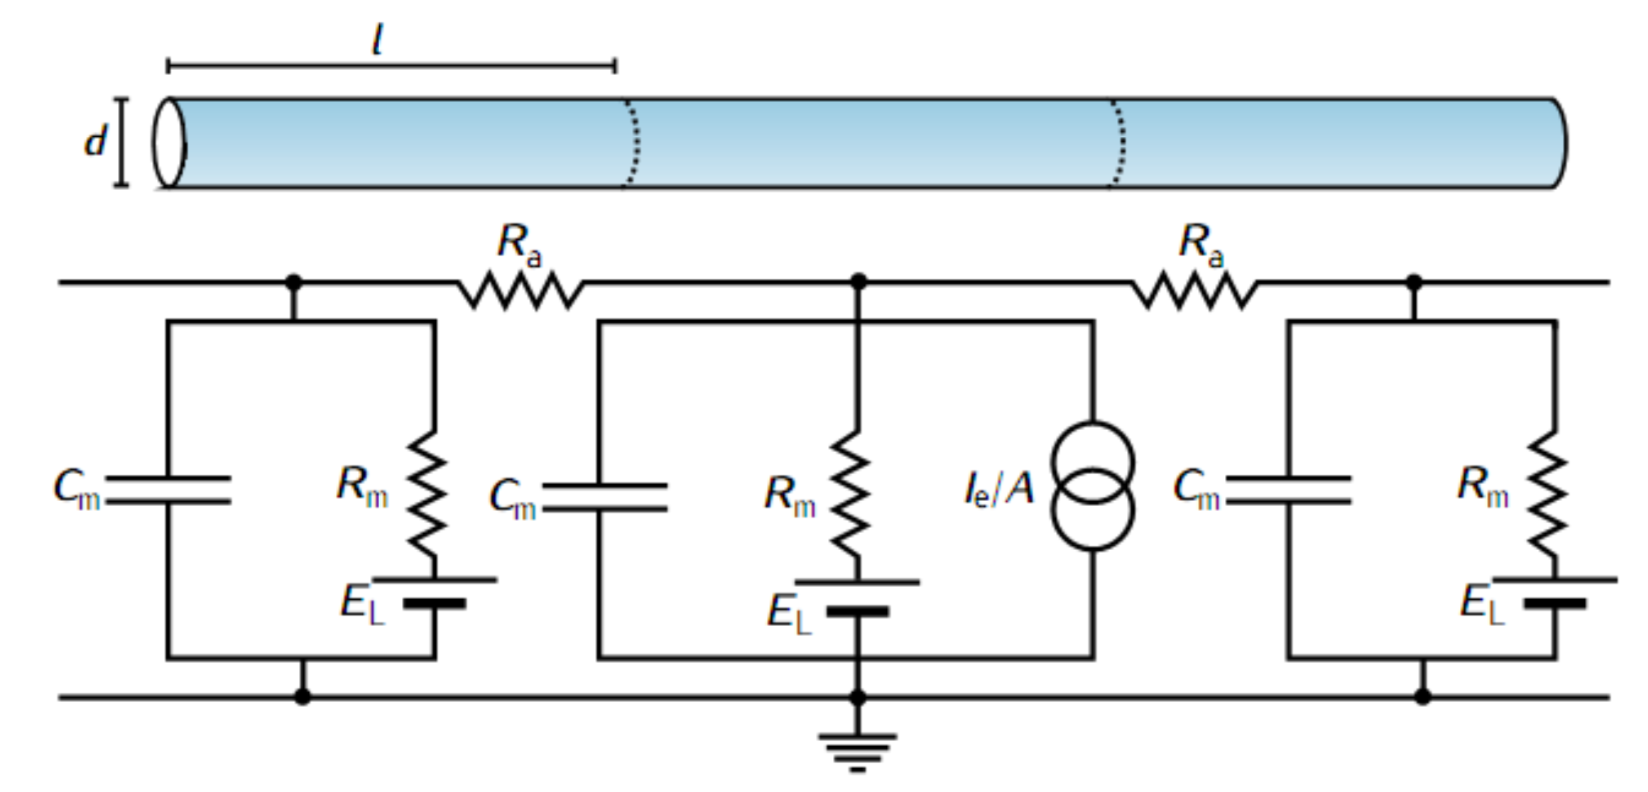
\includegraphics[width=0.7\textwidth]{model.png}
            \caption{Multi-compartment model.}
        \end{figure}
    \item[1.1] In the previous homework we solved for the voltage responses of a two-compartment model. Recall that
    \begin{align*}
        C_{m}\frac{dV_{1}(t)}{dt} &= \frac{E_{m} - V_{1}(t)}{R_m} + \frac{V_{2}(t) - V_{1}(t)}{R_{a}} + I_{e}(t)\\
        C_{m}\frac{dV_{2}(t)}{dt} &= \frac{V_{1}(t) - V_{2}(t)}{R_{a}} + \frac{E_{m} - V_{2}(t)}{R_m}
    \end{align*}
    We need to generalise this to an n-compartment model where $n \geqslant 2$ and arbitrary current $I_{e}(t)$ can be injected into 
    any of the n compartments.\\
    \\
    Following the diagram in Figure 1, we observe that
    $$I_{e, 2}(t) = C_{m}\frac{dV_{2}(t)}{dt} + \frac{V_{2}(t) - E_{L}}{R_{m}} + \frac{V_{2}(t) - V_{3}(t)}{R_{a}} + \frac{V_{2}(t) - V_{1}(t)}{R_{a}}$$
    Where the compartments are labelled 1-3 starting from the right hand side.\\
    \\
    Rearranging yeilds
    $$C_{m}\frac{dV_{2}(t)}{dt} = \frac{E_{L} - V_{2}(t)}{R_{m}} + \frac{V_{3}(t) - V_{2}(t)}{R_{a}} + \frac{V_{1}(t) - V_{2}(t)}{R_{a}} + I_{e, 2}(t)$$
    Note that we have the middle compartment 2 expressed in terms of its neighbouring compartments 1 \& 3. This can thus be generalised as
    $$\frac{dV_{j}(t)}{dt} = \frac{E_{L} - V_{j}(t)}{\tau_{m}} + \frac{1}{C_{m}}\left(\frac{V_{j+1}(t) - V_{j}(t)}{R_{a}} + \frac{V_{j-1}(t) - V_{j}(t)}{R_{a}}\right) + \frac{1}{C_{m}}I_{e, j}(t)$$
    The above equation is known as the fundamental equation of a compartmental model. For the compartments without any current injected the response will look 
    the same but lacking the current term and dependent on the direction of the current flow. 
    Thus, if we use the same numbering scheme, then for compartment i where $0 < i < j$, we have
    $$\frac{dV_{i}(t)}{dt} = \frac{E_{L} - V_{i}(t)}{\tau_{m}} + \frac{1}{C_{m}}\left(\frac{V_{i-1}(t) - 2V_{i}(t) + V_{i+1}(t)}{R_{a}}\right)$$
    Similarly, for compartment i where $j < i < N$ where $N$ is the number of compartments, we have
    $$\frac{dV_{i}(t)}{dt} = \frac{E_{L} - V_{i}(t)}{\tau_{m}} + \frac{1}{C_{m}}\left(\frac{V_{i+1}(t) - 2V_{i}(t) + V_{i-1}(t)}{R_{a}}\right)$$
    \textit{Nota bene} for the terminal compartments (i.e. when $i=0$ or $i=N$ we have to make use of the boundary conditions as 
    shown in Figure 2.
    \begin{figure}[h]
        \centering
        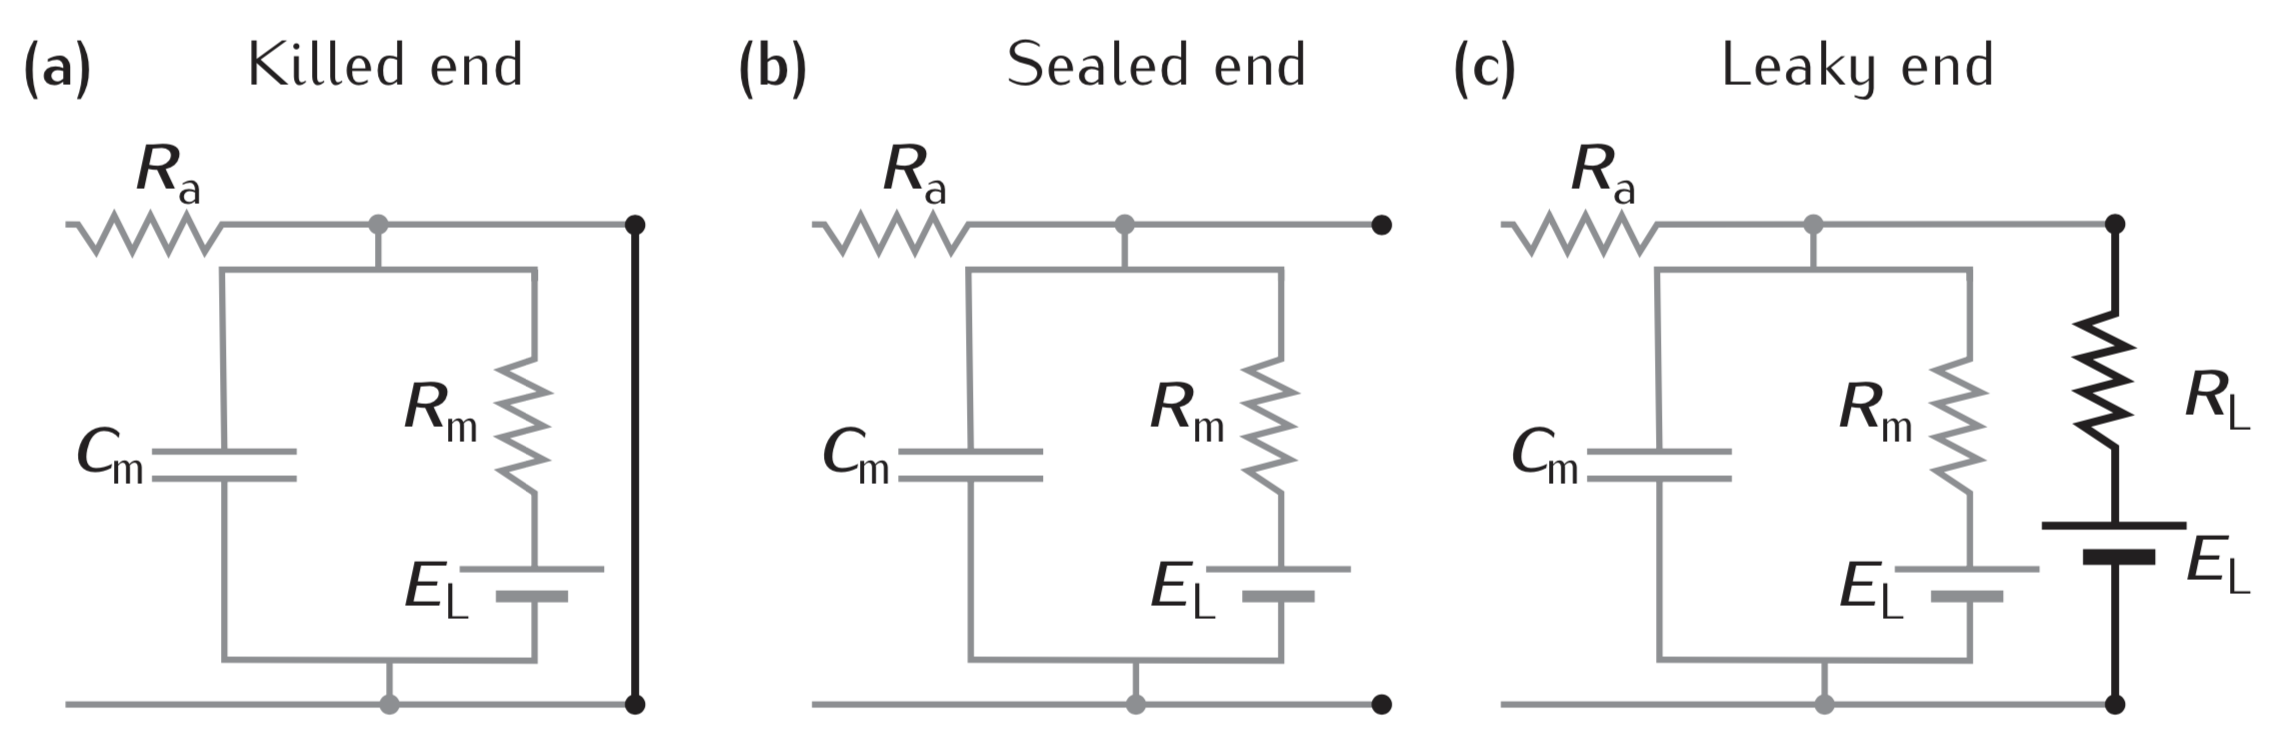
\includegraphics[width=0.9\textwidth]{boundary.png}
        \caption{Boundary conditions for the terminal compartments.}
    \end{figure}
    For the killed end (Dirichlet) boundary condition, the neurite's intracellular environment is in contact with the extracellular medium, 
    and hence the potential $V_{i}$ for that compartment is set to 0, for it is grounded. 
    For the sealed end (Neumann) boundary condition, we assume that the resistance 
    is so high that no current can pass through the end. Since the axial current is proportional to the gradient of the membrane potential, no current 
    implies zero potential gradient.
    \begin{align*}
        \frac{V_{i+1} - V_{i}}{R_{a}} &= C_{m}\frac{dV_{i}}{dt} + \frac{V_{i} - E_{L}}{R_{m}}\\
        \implies \frac{dV_{i}}{dt} &= \frac{E_{L} - V_{i}}{\tau_{m}} + \frac{V_{i+1} - V{i}}{C_{m}R_{a}}
    \end{align*}
    \item[1.2] Equation \ref{eq1} can be approximated with the forward Euler method as shown below
    \begin{align*}
        \frac{V_{j}(t + \Delta t) - V_{j}(t)}{\Delta t} &= \frac{E_{L} - V_{j}(t)}{\tau_{m}} + \frac{1}{C_{m}}\left(\frac{V_{j+1}(t) - V_{j}(t)}{R_{a}} + \frac{V_{j-1}(t) - V_{j}(t)}{R_{a}}\right) + \frac{1}{C_{m}}I_{e, j}(t)
    \end{align*}
    \begin{align*}
        \implies V_{j}(t + \Delta t) = V_{j}(t) &+ \Delta t \left( \frac{E_{L} - V_{j}(t)}{\tau_{m}} + \frac{1}{C_{m}} \left( \frac{V_{j+1}(t) - V_{j}(t)}{R_{a}} + \frac{V_{j-1}(t) - V_{j}(t)}{R_{a}}\right) \right)\\
        &+ \frac{\Delta t}{C_{m}}I_{e, j}(t)
    \end{align*}
    Now, we simulate this with the step current given below 
    \begin{equation} \label{eq1}
    I_{e}(j, t)= 
        \begin{cases}
            0, & (t < t_{e}) \vee (j \neq j_{e})\\
            10 \, \text{pA} ,              & (t_{e} \leqslant t) \wedge (j = j_{e})\\
        \end{cases}
    \end{equation}
    We assume $N = 50$ compartments where the first compartment is terminated as a 'sealed end' 
    and the last compartment is terminated as a 'killed end'. We also assume the following electrical properties
    \begin{enumerate}
        \item[a)] Membrane capacitance $C_{m} = 62.8 \, \text{pF}$
        \item[b)] Membrane resistance $R_{m} = 1.59 \, \text{G\si{\ohm}}$
        \item[c)] Axial resistance $R_{a} = 0.0318 \, \text{G\si{\ohm}}$
        \item[d)] $E_{L} = E_{m} = 0 \, \text{V}$
    \end{enumerate}
    The results of the scenario mentioned above appear in Figure 3.
    \begin{figure}[h]
        \centering
        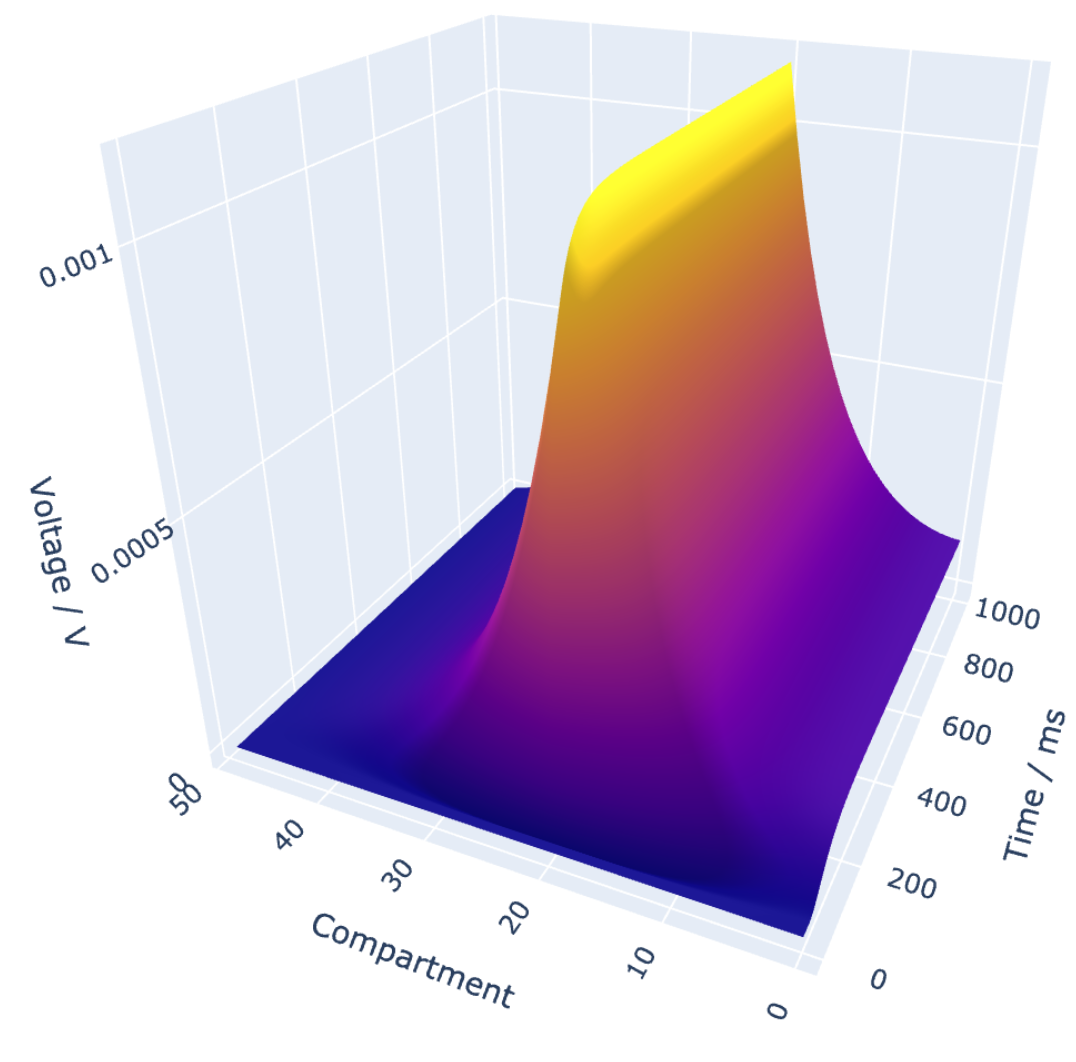
\includegraphics[width=0.7\textwidth]{Figures/fig1_3d.png}
        \caption{Voltage response over time for 50 compartments.}
    \end{figure}
    \item[1.3] As regards the functional form of the spatially-dependent stationary solution $V(j, \infty)$, it 
    decays exponentially while travelling through each compartment away from the current injection site. The voltage decay 
    constant is larger for the current travelling towards the 'sealed end', and hence the voltage decreases slower, as opposed 
    to the other side where it effectively reaches zero.
    \item[1.4] Next, the same multi-compartment model was simulated in response to the rectangular current input
    \begin{equation} \label{eq2}
        I_{e}(j, t)= 
        \begin{cases}
            0, & (t < t_{e}) \vee (t_{s} \leqslant t) \vee (j \neq j_{e})\\
            I_{0}, & (t_{e} \leqslant t < t_{s}) \wedge (j = j_{e})\\
        \end{cases}
    \end{equation}
    with $I_{0}=100 \, \text{pA}$, $j_{e}=14$, $t_{e}=20 \, \text{ms}$, and $t_{s}=200 \, \text{ms}$. The results can be seen in Figure 4.
    \begin{figure}[h]
        \centering
        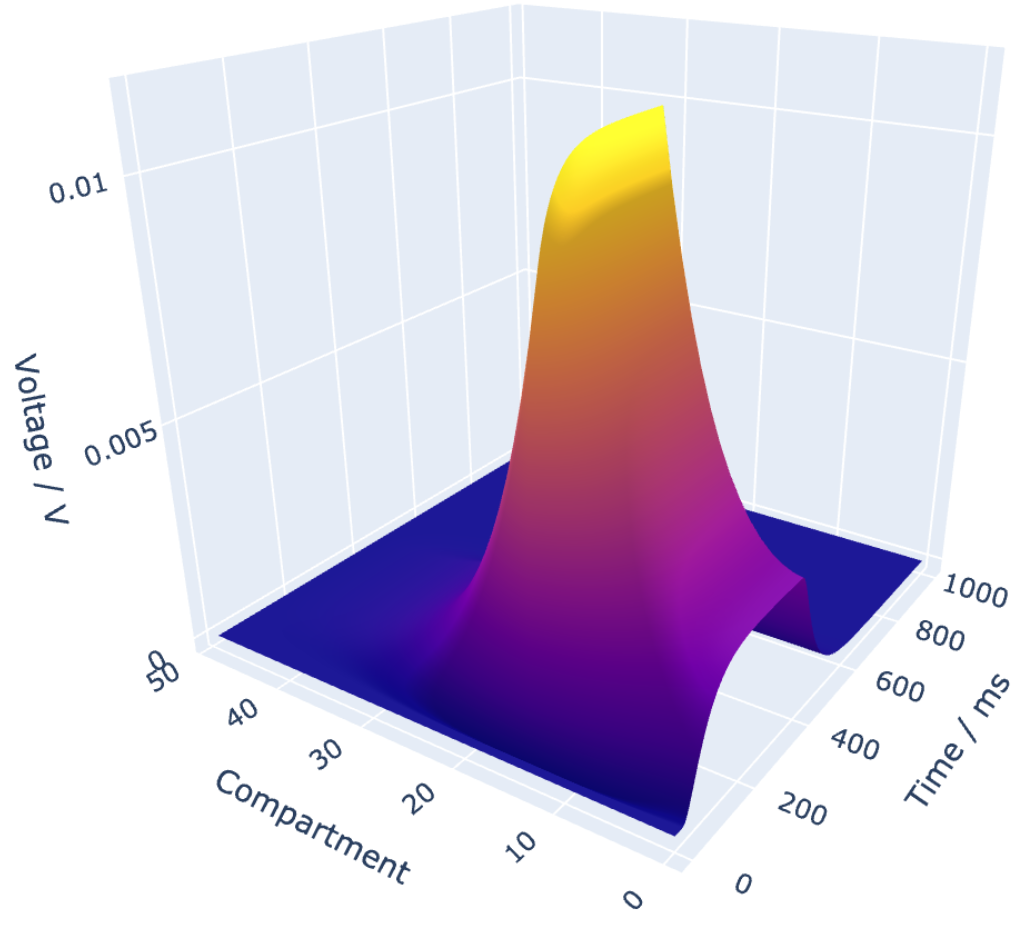
\includegraphics[width=0.7\textwidth]{Figures/fig2_3d.png}
        \caption{Voltage response over time for 50 compartments.}
    \end{figure}
\end{enumerate}

\noindent\textbf{Question 2. Simulation of a single-compartment Hodgkin-Huxley model of an active neurite.}
    \begin{enumerate}
        \item[2.1]
        \begin{figure}[h]
            \centering
            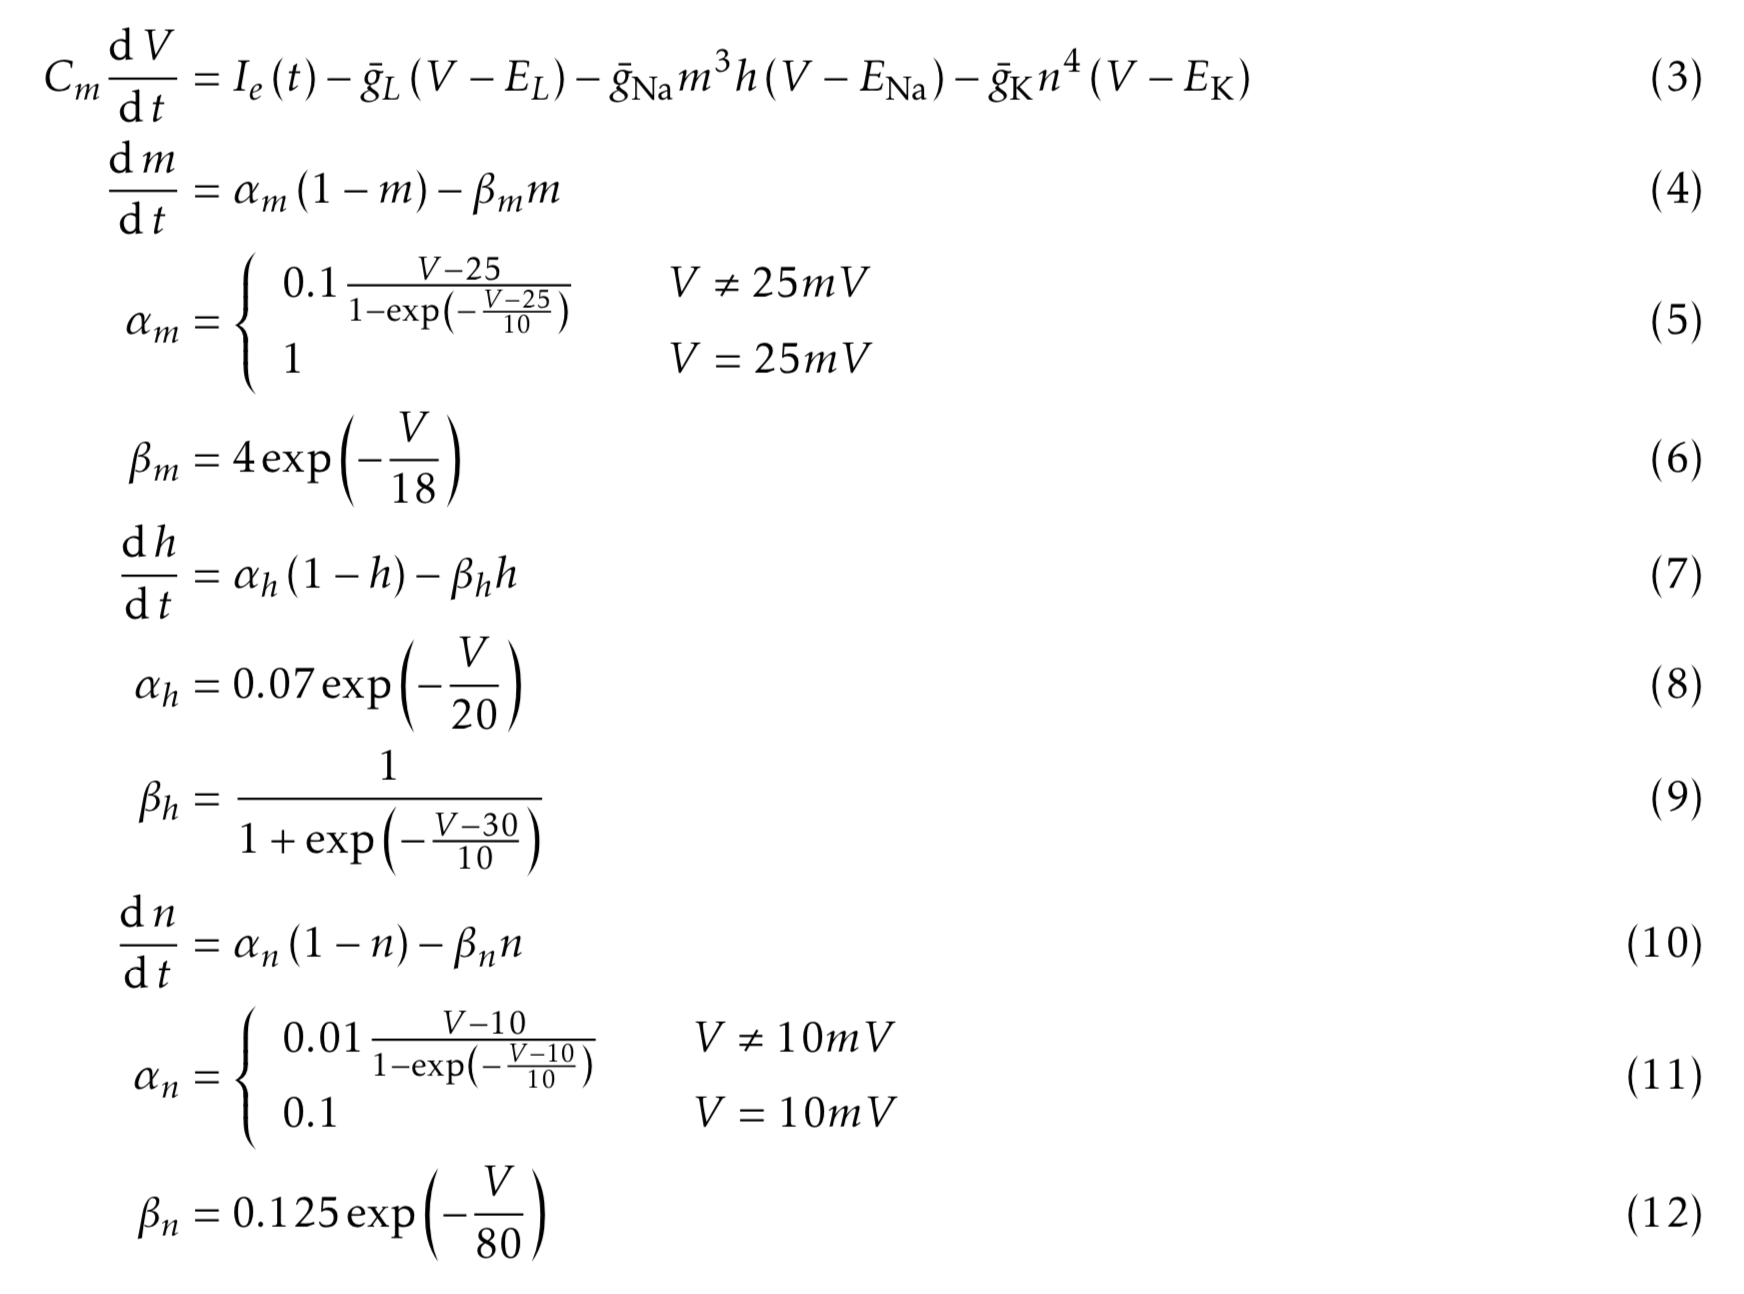
\includegraphics[width=1\textwidth]{Figures/Eqs.png}
        \end{figure} 
        The equations (3-12) give the Hodgkin-Huxley model of an imaginary single-compartment (i.e. no axial current) active neurite with input current $I_{e}(t)$.
        The electric properties for this neurite are
        \begin{itemize}
            \item $C_{m}=1 \, \mu \text{F}$, membrane capacitance
            \item $E_{Na}=115 \, \text{mV}$, sodium equilibrium potential
            \item $E_{K}=-12 \, \text{mV}$, potassium equilibrium potential
            \item $E_{L}=10.6 \, \text{mV}$, leak equilibrium potential
            \item $V(0)=0 \, \text{mV}$, initial membrane potential
            \item $\bar{g}_{Na}=120 \, \text{ms}$, maximum sodium channel conductance
            \item $\bar{g}_{K}=36 \, \text{ms}$, maximum potassium channel conductance
            \item $\bar{g}_{L}=0.3 \, \text{ms}$, maximum leak conductance
        \end{itemize}
        To approximate the given DEQs we will use the Forward Euler method
        \begin{align*}
            V(t + \Delta t) &= V(t) + \frac{\Delta t}{C_{m}}\left(I_{e}(t) - \bar{g}_{L}\left(V(t)-E_{L}\right) - \bar{g}_{Na}m^{3}h\left(V(t)-E_{Na}\right) - \bar{g}_{K}n^{4}\left(V(t)-E_{K}\right)\right)\\
            m(t + \Delta t) &= m(t) + \Delta t\left(\alpha_{m}\left(1-m\right)-\beta_{m}m\right)\\
            h(t + \Delta t) &= h(t) + \Delta t\left(\alpha_{h}\left(1-h\right)-\beta_{h}h\right)\\
            n(t + \Delta t) &= n(t) + \Delta t\left(\alpha_{n}\left(1-n\right)-\beta_{n}n\right)\\
        \end{align*}
        \item[2.2] Now, we implement this model with the input current $I_{e}(t)$ given by equation \ref{eq2} with $t_{e}=50 \, \text{ms}$, 
        $t_{s}=300 \, \text{ms}$ for different amploitudes $I_{0}=0 \, \mu \text{A}$, $I_{0}=3 \, \mu \text{A}$, $I_{0}=6 \, \mu \text{A}$, $I_{0}=8 \, \mu \text{A}$.
        The resulting voltage responses appear in Figures 5, 6, 7, and 8. The code used to generate the following figures appears at the end of the script.
        \begin{figure}[h]
            \centering
            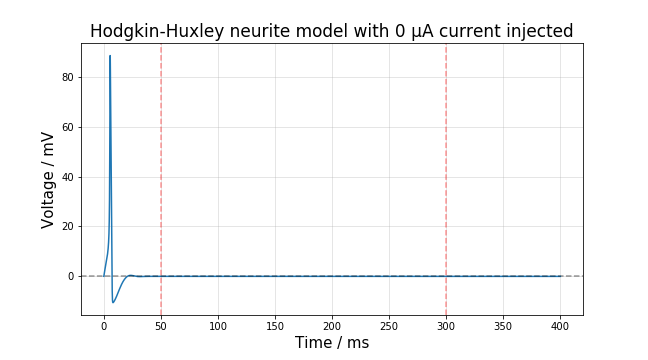
\includegraphics[width=0.9\textwidth]{Current_0A.png}
            \caption{No current injected.}
        \end{figure}
        \begin{figure}[h]
            \centering
            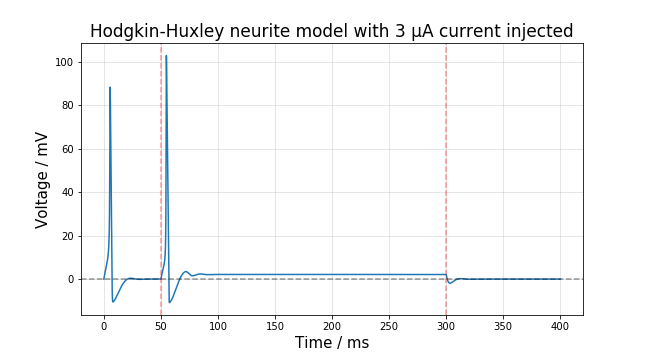
\includegraphics[width=0.9\textwidth]{Current_3A.png}
            \caption{3 $\, \mu \text{A}$ injected.}
        \end{figure}
        \begin{figure}[h]
            \centering
            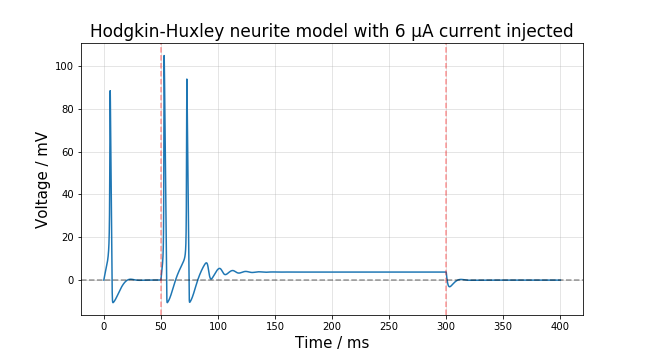
\includegraphics[width=0.9\textwidth]{Current_6A.png}
            \caption{6 $\, \mu \text{A}$ injected.}
        \end{figure}
        \begin{figure}[h]
            \centering
            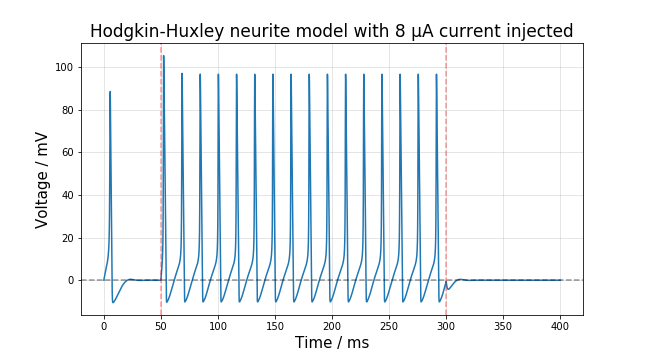
\includegraphics[width=0.9\textwidth]{Current_8A.png}
            \caption{8 $\, \mu \text{A}$ injected.}
        \end{figure}
        \item[2.3] Next, we simulate the model with different amplitudes of input 
        current (from $I_{0}=0 \, \mu \text{A}$ to $I_{0}=20 \, \mu \text{A}$) in steps of $0.5 \, \mu \text{A}$. 
        The plot of firing rate in the stationary state ($200 \, \text{ms}$ after current injection) plotted against applied current is shown in Figure 9.
        \begin{figure}[h]
            \centering
            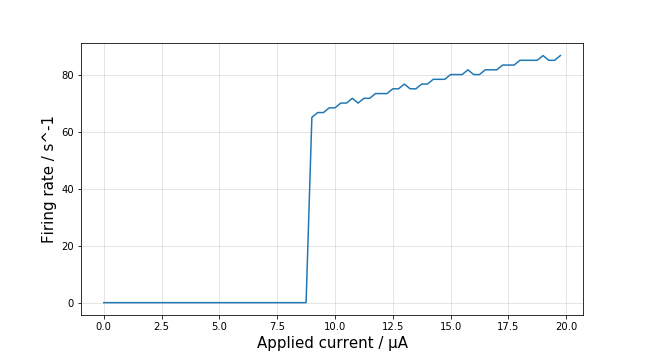
\includegraphics[width=0.9\textwidth]{Firing_rate.png}
            \caption{Elicited firing rate in response to applied currenr of varying amplitude.}
        \end{figure}
    \end{enumerate}
\end{document}
